%%%%%%%%%%%%%%%%%%%%%%%%%%%%%%%%%%%%%%%%%
% * <licancanair@gmail.com> 2017-09-25T23:23:17.943Z:
%
% ^.
%
%%%%%%%%%%%%%%%%%%%%%%%%%%%%%%%%%%%%%%%%%

%----------------------------------------------------------------------------------------
%	PACKAGES AND THEMES
%----------------------------------------------------------------------------------------

\documentclass{beamer}
\mode<presentation> {
% The Beamer class comes with a number of default slide themes
% which change the colors and layouts of slides. Below this is a list
% of all the themes, uncomment each in turn to see what they look like.

%\usetheme{default}
%\usetheme{AnnArbor}
%\usetheme{Antibes}
%\usetheme{Bergen}
%\usetheme{Berkeley}
%\usetheme{Berlin}
%\usetheme{Boadilla}
\usetheme{CambridgeUS}
%\usetheme{Copenhagen}
%\usetheme{Darmstadt}
%\usetheme{Dresden}
%\usetheme{Frankfurt}
%\usetheme{Goettingen}
%\usetheme{Hannover}
%\usetheme{Ilmenau}
%\usetheme{JuanLesPins}
%\usetheme{Luebeck}
%\usetheme{Madrid}
%\usetheme{Malmoe}
%\usetheme{Marburg}
%\usetheme{Montpellier}
%\usetheme{PaloAlto}
%\usetheme{Pittsburgh}
%\usetheme{Rochester}
%\usetheme{Singapore}
%\usetheme{Szeged}
%\usetheme{Warsaw}

% As well as themes, the Beamer class has a number of color themes
% for any slide theme. Uncomment each of these in turn to see how it
% changes the colors of your current slide theme.

%\usecolortheme{albatross}
%\usecolortheme{beaver}
%\usecolortheme{beetle}
%\usecolortheme{crane}
%\usecolortheme{dolphin}
%\usecolortheme{dove}
%\usecolortheme{fly}
%\usecolortheme{lily}
%\usecolortheme{orchid}
%\usecolortheme{rose}
%\usecolortheme{seagull}
%\usecolortheme{seahorse}
%\usecolortheme{whale}
%\usecolortheme{wolverine}

%\setbeamertemplate{footline} % To remove the footer line in all slides uncomment this line
%\setbeamertemplate{footline}[page number] % To replace the footer line in all slides with a simple slide count uncomment this line

%\setbeamertemplate{navigation symbols}{} % To remove the navigation symbols from the bottom of all slides uncomment this line
}

\usepackage{graphicx} % Allows including images
\usepackage{booktabs} % Allows the use of \toprule, \midrule and \bottomrule in tables
\usepackage{dsfont}
\usepackage{hyperref}
\usepackage{dirtytalk}
\usepackage{graphicx}
\usepackage{caption}
\usepackage{subcaption}
%\usepackage{times}
\usepackage{tikz}
\usepackage{verbatim}
\usetikzlibrary{arrows,shapes}
\newcommand{\sigmoid}{\ensuremath{\sigma(\theta^T \textbf{x})}}
\usepackage{multicol}
\usepackage{ amssymb }
\usepackage{amsmath,amsfonts,amsthm,bm} % Math packages
\DeclareMathAlphabet{\mathbbm}{U}{bbm}{m}{n}
%----------------------------------------------------------------------------------------
%	TITLE PAGE
%----------------------------------------------------------------------------------------

\title[Logistic Regression]{Logistic Regression} % The short title appears at the bottom of every slide, the full title is only on the title page

\author{Wenzhen Zhu, Sayantan Bhadra, Cancan Li, Charlie Wu, Chih Yun Pai} % Your name
\institute[WUSTL] % Your institution as it will appear on the bottom of every slide, may be shorthand to save space
{
Washington University in St. Louis \\ % Your institution for the title page
\medskip
\textit{CSE 543T Algorithms for Nonlinear Optimization} % Class Number
}
\date{September 26, 2017} % Date, can be changed to a custom date

\begin{document}

\begin{frame}
\titlepage % Print the title page as the first slide
\end{frame}

\begin{frame}
\frametitle{Overview} % Table of contents slide, comment this block out to remove it
\tableofcontents % Throughout your presentation, if you choose to use \section{} and \subsection{} commands, these will automatically be printed on this slide as an overview of your presentation
\end{frame}

%----------------------------------------------------------------------------------------
%	PRESENTATION SLIDES
%----------------------------------------------------------------------------------------

\section{Introduction}

\begin{frame}
\huge{\centerline{Section 1: Introduction }}
\end{frame}
\begin{frame}
\frametitle{Binary Classification} % Table of contents slide, comment this block out to remove it
\begin{itemize}
\item Key problem in supervised machine learning.


%----------------------------------------------------------------------------------------
%	PRESENTATION SLIDES
%----------------------------------------------------------------------------------------

%------------------------------------------------
\item Predict binary output from input variables, e.g.
%Examples:
\begin{itemize}
\item[--] Spam or not spam
\item[--] Disease or no disease
\item[--] Rain or no rain
\item[--] Win or lose election etc.
\end{itemize}
%\section{Binary classification} % Sections can be created in order to organize your presentation into discrete blocks, all sections and subsections are automatically printed in the table of contents as an overview of the talk
%------------------------------------------------

%\subsection{Spam or not spam} % A subsection can be created just before a set of slides with a common theme to further break down your presentation into chunks
%\subsection{Disease or no disease etc.}
\item Simplest classifiers: linear classifiers, e.g. \textit{perceptron}.
\end{itemize}
\end{frame}
%------------------------------------------------
\begin{frame}
\frametitle{Linear classification}
\begin{figure}
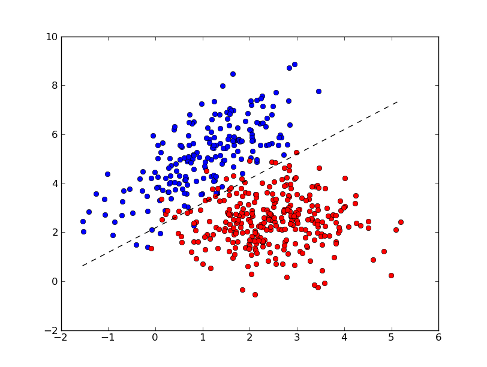
\includegraphics[width=0.6\linewidth]{lda_binary.png}
\caption{Example of linear classification}
\end{figure}
\end{frame}
%------------------------------------------------
\begin{frame}
\frametitle{Linear Classification}
\begin{itemize}
\item Output binary class (0 or 1) based on where a linear combination of the input feature vector lies with respect to the decision boundary:
\begin{equation}
y = \frac{1}{2}(1 + \text{sign} (\theta^T \mathbf{x}))
\end{equation}
$\mathbf{x} \in \mathds{R}^{d+1}, \theta \in \mathds{R}^{d+1}; y \in \{0,1\}.$\\

\begin{itemize}
\item[--] $ \theta^T \mathbf{x} = 0 \implies \text{decision boundary}$
\item[--] $ \theta^T \mathbf{x} > 0 \implies y = 1$
\item[--] $ \theta^T \mathbf{x}  < 0 \implies y = 0$
\end{itemize}

\item The decision boundary (i.e. $\theta$) is learned from the training data.
\end{itemize}
\end{frame}

\begin{frame}
\frametitle{Hard vs. Soft Threshold}
\begin{itemize}
\item Exact binary prediction (\textit{hard threshold}) may be impractical - does not reveal the confidence in the prediction.
% Talk about the non-linearity as well
\item Express as \textit{probability} of belonging to a class (\textit{soft threshold}), e.g. probability of raining, probability of a heart disease etc. \item Instead of a strict binary value, the classifier output is a real number between 0 and 1 - interpreted as class probability.
\item This leads to \textbf{logistic regression}.
\end{itemize}
\end{frame}

\begin{frame}
\frametitle{Modeling Conditional Probabilities}
\begin{itemize}
\item Determine a conditional probability distribution, or \textit{likelihood} $P(Y|X)$ that best describes the observed data.
\item Assuming $P(Y=1|X=\mathbf{x}) = p(\mathbf{x};\theta)$ for some function $p$ parameterized by $\theta$ and with $i.i.d.$ observation variables, the conditional likelihood function $P(Y|X)$ is,
\begin{equation}
\prod_{i=1}^n P(Y=y_i|X=\mathbf{x}_i) = \prod_{i=1}^n p(\mathbf{x}_i;\theta)^{y_i} (1-p(\mathbf{x}_i;\theta)^{1-y_i})
\end{equation}
\item Estimate $\theta$ by \textit{maximum likelihood estimation}.  
\end{itemize}
\end{frame}

%----------------------------------------------------------------------------------------
%	PRESENTATION SLIDES Section 2
%----------------------------------------------------------------------------------------
\section{Logistic Regression} 

\begin{frame}
\huge{\centerline{Section 2: Logistic Regression Model}}
\end{frame}
%------------------------------------------------
\subsection{Iris Flower}
\begin{frame}
\frametitle{Fisher's Iris}
The data set consists of 50 samples from each of three 
species of iris flowers.  Four features were measured from each
sample, they are the length and the width of sepal and petal. This data set is often used
to demonstrate classification techniques and discriminant analysis.

\begin{figure}
\centering
\begin{subfigure}{.3\textwidth}
  \centering
  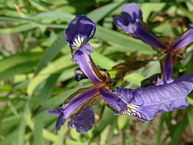
\includegraphics[scale=.45]{graphics/setosa}
  \caption{setosa}
  \label{fig:sub1}
\end{subfigure}%
\begin{subfigure}{.3\textwidth}
  \centering
  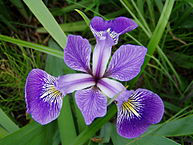
\includegraphics[scale=.45]{graphics/versicolor}
  \caption{versicolor}
  \label{fig:sub2}
\end{subfigure}
% 
\begin{subfigure}{.3\textwidth}
  \centering
  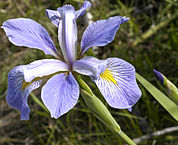
\includegraphics[scale=.45]{graphics/virginica}
  \caption{virginica}
  \label{fig:sub2}
\end{subfigure}
\label{fig:test}
\end{figure}


\end{frame}

%------------------------------------------------
\begin{frame}
\frametitle{Fisher's Iris}
Four features were measured from each
sample, they are the length and the width of sepal and petal.
\begin{figure}[htbp]
\centering
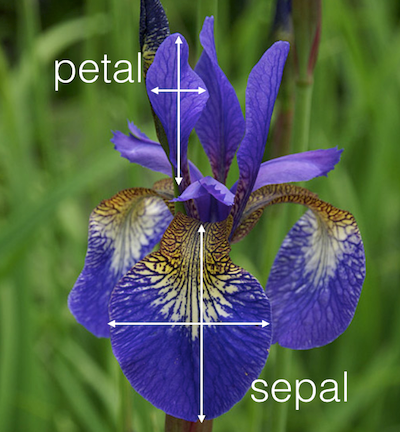
\includegraphics[scale=.35]{graphics/iris_feature} \caption{Features}
\label{fig:Features}
\end{figure}
\end{frame}
%------------------------------------------------
\begin{frame}
\frametitle{Sample Data}

\begin{table}
\begin{tabular}{lllll}
\hline
\textbf{Sepal Length} & \textbf{ Sepal Width } & \textbf{Petal Length} & \textbf{Petal Width} & \textbf{Species}\\
\hline
5.8 & 4.0 & 1.2 & 0.2 & setosa\\
6.4 & 2.8 & 5.6 & 2.1 & virginica\\
6.7 & 3.1 & 5.6 & 2.4 & virginica \\
\hline
\end{tabular}
\caption{Fisher's Iris Dataset Sample}
\end{table}

\begin{figure}[htbp]
\centering
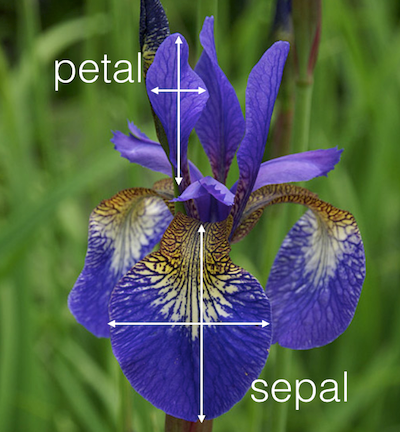
\includegraphics[scale=.23]{graphics/iris_feature} \caption{Features}
\end{figure}


\end{frame}
%------------------------------------------------
\begin{frame}
\frametitle{Visualization of Iris Dataset}
\begin{figure}[t]
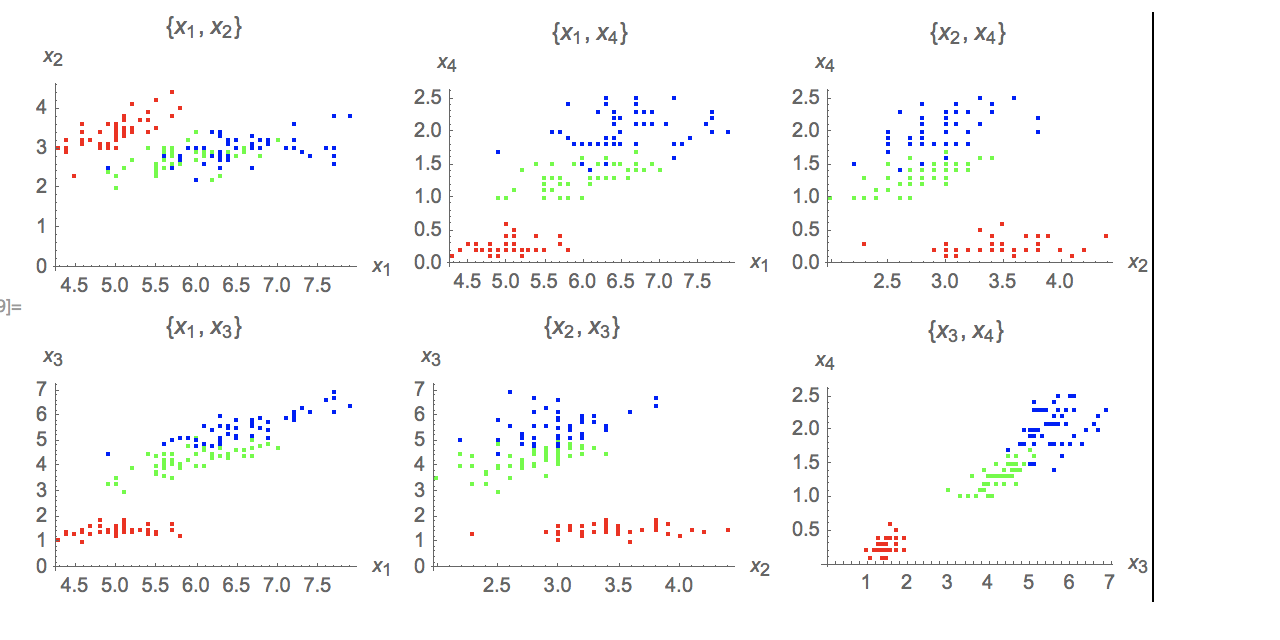
\includegraphics[scale=0.5]{graphics/feature_vis}
\centering
\end{figure}
\end{frame}
%------------------------------------------------
\begin{frame}
\frametitle{}
\[\text{Let's start from binary classification y $\in $ $\{$0, 1$\}$}\]

\[\text{y $\in $ $\{$0, 1$\}$   where 0 $\to $ versicolor 1$\to $ virginica}\]
\[	
	\mathbf{x} = (x_ 1, x_ 2) \
		where \ x_1 = \text{sepal width}, x_2 = \text{petal width}\]
		
% ----------
\begin{figure}
\begin{subfigure}{.4\textwidth}
  \centering
  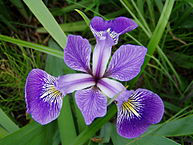
\includegraphics[scale=.5]{graphics/versicolor}
  \caption{versicolor}
  \label{fig:sub1}
\end{subfigure}
% 
\begin{subfigure}{.4\textwidth}
  \centering
  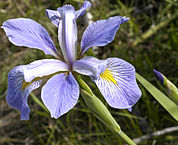
\includegraphics[scale=.5]{graphics/virginica}
  \caption{virginica}
  \label{fig:sub2}
\end{subfigure}
\label{fig:test}
\end{figure}
% ----------
\end{frame}
%------------------------------------------------
\subsection{Sigmoid Function}
\begin{frame}
\frametitle{Sigmoid Function}
\[\sigma(x)=\frac{1}{1+e^{-x}}\]
\begin{figure}[t]
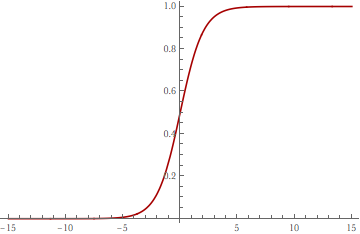
\includegraphics[width=5cm]{graphics/1d-sigmoid}
\centering
\end{figure}
\end{frame}
%------------------------------------------------
\begin{frame}
\begin{multicols}{2} % 2 columns
\begin{figure}[t]
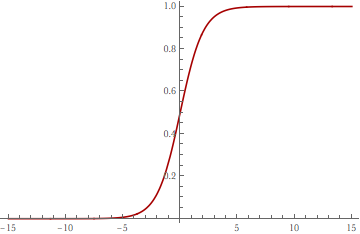
\includegraphics[width=5cm]{graphics/1d-sigmoid}
\centering
\end{figure}
\columnbreak  % seperate
In this example, you can think 
\[ \bm{\theta} = (\theta_{0}, \theta_{1}) \ and \ \mathbf{x} = (1, x)\]
therefore, 
\[p(\mathbf{x} ;  \bm{\theta}) =  \frac{1}{1+e^{- ( \theta_{0} +  \theta_{1} \cdot  x )}} \]
\\
\end{multicols}
\begin{multicols}{2}
\[p(x;  \bm{\theta}) \geq \frac{1}{2}  \Rightarrow class 1\]
\[p(x;  \bm{\theta})<\frac{1}{2}  \Rightarrow class 0\]
\columnbreak 
\[p(\mathbf{x};  \bm{\theta})=P(y=1|\mathbf{x}) = \frac{1}{1+e^{-\bm{\theta} ^ {\intercal} \mathbf{x}}}\]
\[1-p(\mathbf{x};  \bm{\theta})=P(y=0|\mathbf{x}) = \frac{e^{-\bm{\theta} ^ {\intercal} \mathbf{x}}} {1+e^{-\bm{\theta}^\intercal \mathbf{x}}} \]
\end{multicols}
\end{frame}
%------------------------------------------------ 
\begin{frame}
\begin{centering}
\begin{equation}
\begin{aligned}
class 1 &\Leftrightarrow p(\mathbf{x};  \bm{\theta}) = \frac{1}{1+e^{-\bm{\theta} ^ {\intercal} \mathbf{x}}} > \frac{1}{2} \\
&\Leftrightarrow e^ {-\bm{\theta} ^ {\intercal} \mathbf{x}} > 1\\
&\Leftrightarrow \bm{\theta} ^ {\intercal} \mathbf{x} > 0\\
\end{aligned}
\end{equation}
\\
\begin{equation}
\begin{aligned}
class 0 &\Leftrightarrow p(\mathbf{x};  \bm{\theta}) = \frac{1}{1+e^{-\bm{\theta} ^ {\intercal} \mathbf{x}}} < \frac{1}{2} \\
&\Leftrightarrow e^ {-\bm{\theta} ^ {\intercal} \mathbf{x}} < 1\\
&\Leftrightarrow \bm{\theta} ^ {\intercal} \mathbf{x} < 0\\
\end{aligned}
\end{equation}
\end{centering}
%\[p(\mathbf{x}) = \frac{1}{1+e^{-\bm{\theta \intercal} \mathbf{x}}} \geq \frac{1}{2} \Leftrightarrow \bm{\theta \intercal} \mathbf{x} > 0 \Rightarrow class 1\]
%\[p(\mathbf{x}) = \frac{1}{1+e^{-\bm{\theta \intercal} \mathbf{x}}} <\frac{1}{2}  \Leftrightarrow \bm{\theta \intercal} \mathbf{x} < 0 \Rightarrow class 0\]
\\
\begin{block}{Conclusion}
\begin{itemize}
\item Logistic regression gives us a \textbf{linear classifier}. \\
\item $\bm{\theta}  ^\intercal \mathbf{x} = 0$ is \textbf{decision boundary}. 
\end{itemize}
\end{block}
\end{frame}
%------------------------------------------------
\begin{frame}
3D Visualization \\
See a Mathematica Dynamic Visualization
\end{frame}
%------------------------------------------------
\subsection{Likelihood Function for Logistic Regression}
\begin{frame}
\frametitle{Maximum Likelihood}

We can assume that
\[P(y = 1 | \mathbf{x}) = p(\mathbf{x}; \bm{\theta})\]
\[P(y = 0 | \mathbf{x}) = 1- p(\mathbf{x}; \bm{\theta})\]

The likelihood function $\mathcal{L}$, which quantifies how likely output is given input, is defined as follows:
% likelihood
\begin{equation}
\begin{aligned}
\mathcal{L}(\bm{\theta}) &= \prod_{i=1}^n P(Y = y_{i}  | X = \mathbf{x}_{i}; \bm{\theta}) = \prod_{y_{i} = 0 } (1-p(\mathbf{x}_{i}; \bm{\theta})) \prod_{y_{i} = 1 } (p(\mathbf{x}_{i}; \bm{\theta})) \\
&= \prod_{i=1}^{n} p(\mathbf{x}_{i}; \bm{\theta})^{y_{i}} (1-p(\mathbf{x}_{i}; \bm{\theta}))^{(1-{y_{i}})}
\end{aligned}
\end{equation}
\end{frame}

%------------------------------------------------
\begin{frame}
\frametitle{Maximum Likelihood}

% likelihood
\begin{equation}
\begin{aligned}
\mathcal{L}(\bm{\theta}) &= \prod_{i=1}^n P(Y = y_{i}  | X = \mathbf{x}_{i}, \bm{\theta}) = \prod_{y_{i} = 0 } (1-p(\mathbf{x}_{i}; \bm{\theta})) \prod_{y_{i} = 1 } (p(\mathbf{x}_{i}; \bm{\theta})) \\
&= \prod_{i=1}^{n} p(\mathbf{x}_{i}; \bm{\theta})^{y_{i} }(1-p(\mathbf{x}_{i}; \bm{\theta}))^{(1-{y_{i}})}
\end{aligned}
\end{equation}

\begin{equation}
\begin{aligned}
\ell (\bm{\theta}) &=  \log (\mathcal{L}(\bm{\theta}) ) = \sum_{i=1}^{n} y_{i} \log(p(\mathbf{x}_{i}; \bm{\theta}) + (1-y_{i}) \log(1-p(\mathbf{x}_{i}; \bm{\theta})) \\
&= \sum_{y_{i} = 0 } \log (1-p(\mathbf{x}_{i}; \bm{\theta})) + \sum_{y_{i} = 1} \log (p(\mathbf{x}_{i}; \bm{\theta})) \\
\end{aligned}
\end{equation}

Since $f(x) = log(x)$ is a monotonically increasing function, maximizing $\mathcal{L}(\bm{\theta})$ is equivalent as maximizing $\ell(\bm{\theta})$
\end{frame}
%------------------------------------------------
\begin{frame}
\frametitle{Maximum Likelihood Estimation}
Set derivatives equal to zero, then solve, we will find the maximum likelihood.
Let $p(\mathbf{x}) = \sigma(\bm{\theta}^{\intercal} \mathbf{x}) = \frac{1}{1+ e^{-\bm{\theta}^{\intercal} \mathbf{x}}}$

\begin{equation}
\begin{aligned}
\ell'(\bm{\theta}) 
&= \frac{\partial \ell}{\partial \bm{\theta}} =\left(y \frac{1}{\sigma(\bm{\theta}^{\intercal} \mathbf{x})} - (1-y) \frac{1}{1-\sigma(\bm{\theta}^{\intercal} \mathbf{x})}\right) 
\frac{\partial }{\partial \bm{\theta}_{j}} \sigma(\bm{\theta}^{\intercal} \mathbf{x}) \\
&= \left(y \frac{1}{\sigma(\bm{\theta}^{\intercal} \mathbf{x})} - (1-y) \frac{1}{1-\sigma(\bm{\theta}^{\intercal} \mathbf{x})}\right) 
\sigma(\bm{\theta}^{\intercal} \mathbf{x})(1-\sigma(\bm{\theta}^{\intercal} \mathbf{x})) 
\frac{\partial }{\partial \bm{\theta}_{j}} \bm{\theta}^{\intercal} \mathbf{x} \\
&= \left(y(1-\sigma(\bm{\theta}^{\intercal} \mathbf{x}) - (1-y) \sigma(\bm{\theta}^{\intercal} \mathbf{x}) \right) \mathbf{x}_{j} \\
&= (y - p(\mathbf{x}))\mathbf{x}_{j}
\end{aligned}
\end{equation}

Solve for $\bm{\theta}$ by setting $\ell'(\bm{\theta}) =0$ \\
Let's go back to our iris flower and take a look of a concrete example!
\end{frame}
%------------------------------------------------
\subsection{Logistic Regression with More Than Two Classes}
\begin{frame}
\frametitle{Logistic Regression with More Than Two Classes}
If $Y$ can take on $k$ values, i.e. we have $k$ classes, we can still use logistic regression. The predicted conditional probabilities will be 
\begin{equation}
P(Y = c | X = \mathbf{x}) = \frac{\exp ({{\bm{\theta}}^{c}}^ {\intercal} \mathbf{x})} { \sum_{j}^{k} \exp({{\bm{\theta}}^{j}}^ {\intercal}\mathbf{x}) }
\end{equation}
This is commonly known as Softmax function.
\end{frame}
%------------------------------------------------
\subsection{More Topics About Logistic Regression}
\begin{frame}
\large{\centerline{More topics about logistic regression..}}
\end{frame}

%----------------------------------------
% The Math of March Madness
%--------------------------------------
% Frame 1
\begin{frame}
\frametitle{The Math of March Madness}
\begin{figure}
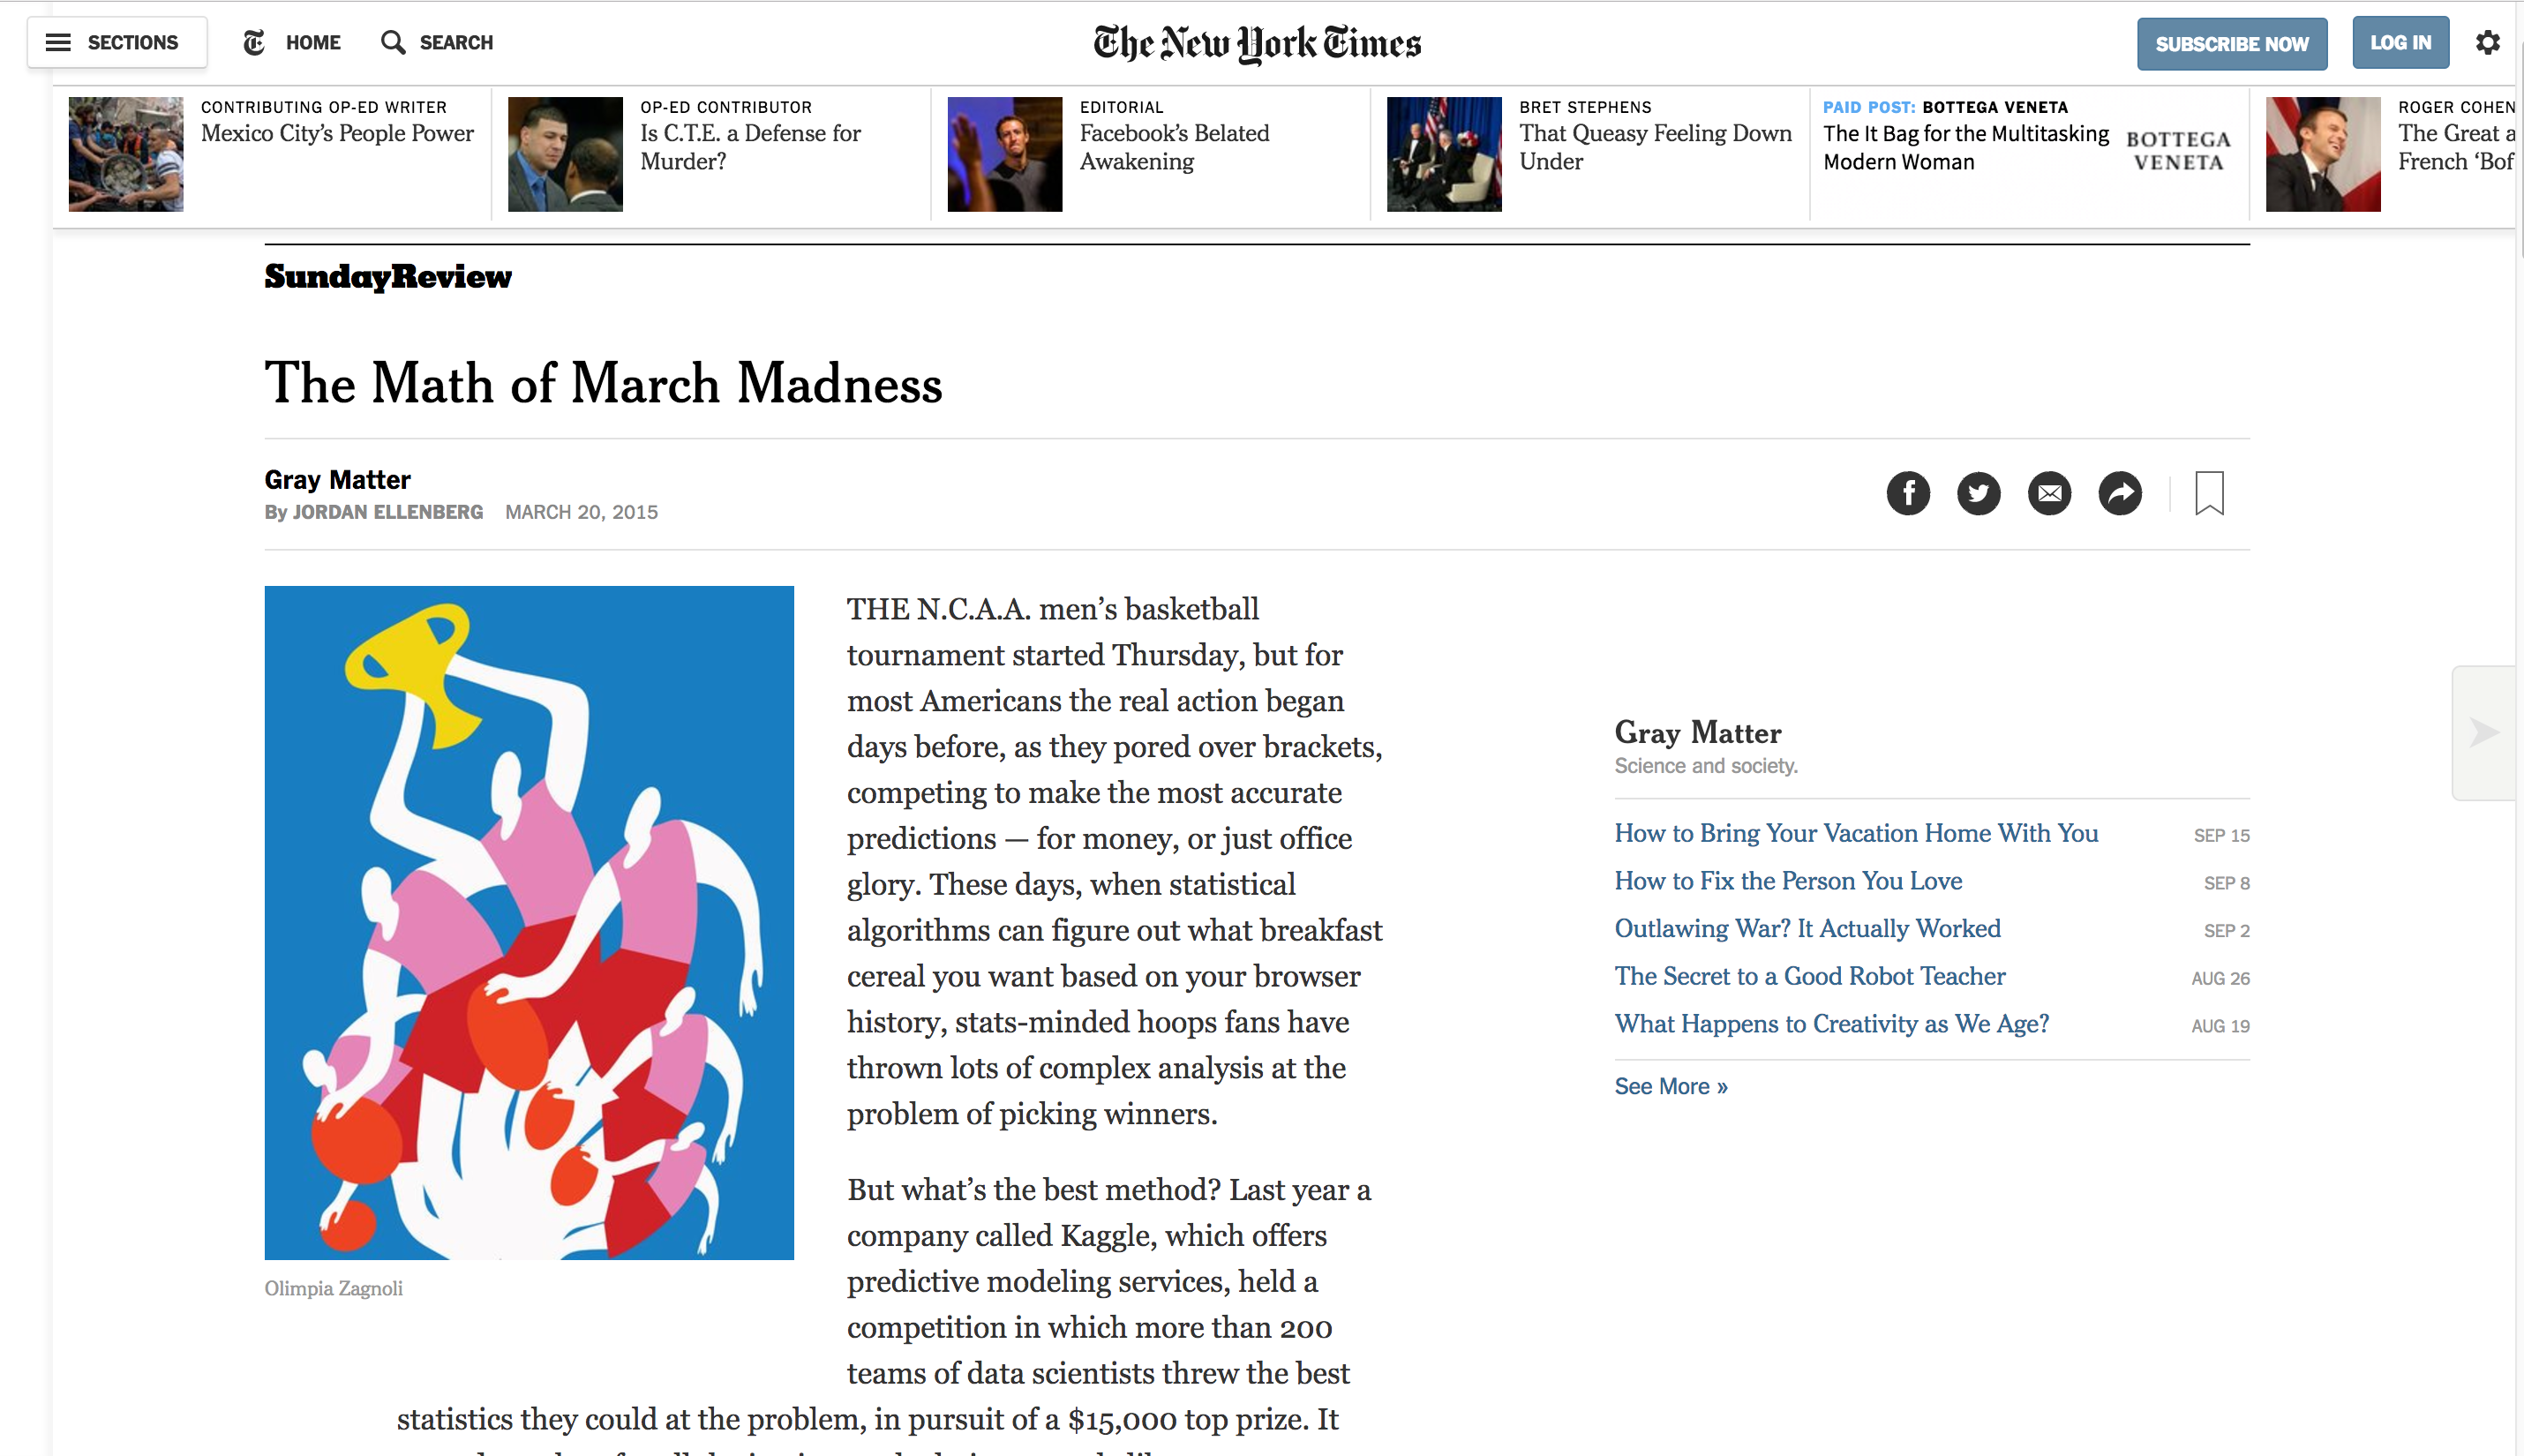
\includegraphics[width=0.8\linewidth]{Math_of_march_madness.png}
\end{figure}
\end{frame}

% Frame 2
\begin{frame}
\frametitle{The Math of March Madness}
\begin{itemize}
\item \say{\textit{Professors Lopez and Matthews didn't use any of the au courant methods in data science circles, either: no deep learning, no hierarchical clustering, no compressed sensing; just a good old model called \textbf{logistic regression}, which turns a number (like a point spread) into an estimated probability that team A will beat team B.}}
\end{itemize}
\end{frame}

% Frame 3
\begin{frame}
\frametitle{The Math of March Madness}
\begin{itemize}
\item Just 2 data sources used - the Las Vegas point spreads for the N.C.A.A. match-ups and a set of offensive and defensive efficiency ratings. 
\item Shows that if the data is simple, then logistic regression can be an efficient algorithm - compared to more complex methods which may easily overfit.
\end{itemize}
\end{frame}

% --------------------------
% Relation with cross-entropy
% --------------------------
% Frame 1
\begin{frame}
\frametitle{Relation with Cross-entropy Error Measure}
\begin{itemize}
\item For two probability distributions $\{p,1-p\}$ and $\{q,1-q\}$ with binary outcomes, the \textit{cross-entropy} (from information theory) 
\begin{equation}
\begin{split}
&= p \log \frac{1}{q} + (1-p) \log \frac{1}{1-q}\\
&= -p \log q - (1-p) \log (1-q)
\end{split}
\end{equation}
\item Assuming that $p$ is the \say{true} distribution and $q$ is the approximate distribution for $p$, minimizing the cross-entropy is equivalent to minimizing the distance (KL-divergence) between the 2 distributions,  i.e. make the approximate distribution as close to the "true" distribution as possible.
\end{itemize}
\end{frame}

% Frame 2
\begin{frame}
\frametitle{Relation with Cross-entropy Error Measure}
\begin{itemize}
\item For the $i^{th}$ training data,
\begin{equation}
\begin{split}
p_i &= y_i \\
q_i &= \sigma (\theta^T \mathbf{x}_i)
\end{split}
\end{equation}
\item The negative log likelihood for the $i^{th}$ training data point may be expressed as
\begin{equation}
-\log P(Y=y_i|X=\mathbf{x_i}) = -y_i \log \sigma (\theta^T \mathbf{x}_i) - (1-y_i) \log (1-\sigma (\theta^T \mathbf{x}_i))
\end{equation}
\item Same as cross-entropy measure.
\end{itemize}
\end{frame}

% Frame 3
\begin{frame}
\frametitle{Relation with Cross-entropy Error Measure}
\begin{itemize}
\item Total cross-entropy error measure over all data points is equal to the negative log likelihood for observation $Y$ given training data set $\mathbf{x}$ and $\theta$, i.e. the cost function for the logistic regression model.
\item Minimizing the cost function w.r.t. $\theta$ may thus be also interpreted as minimizing the distance between the \say{true} distribution (i.e. observation) and the sigmoid approximation.

\end{itemize}
\end{frame}


%------------------------------------------------
% Regularization
%------------------------------------------------
% Frame 1
\subsection{Regularization}
\begin{frame}
\frametitle{Regularization}
\begin{itemize}
\item \textbf{Bayesian view:} If the parameters are assumed to have a prior distribution, then we need to perform \textit{maximum a posteriori} (MAP) estimation.
\item Recall, Bayes' theorem:
\begin{equation}
posterior \propto likelihood \times prior
\end{equation}
\item If the parameters are assumed to have a prior distribution, then we need to perform \textit{maximum a posteriori} (MAP) estimation.
\end{itemize}
\end{frame}
%--------------------------------------------------
\begin{frame}
\frametitle{Regularization}
\begin{itemize}
\item Let $P(\mathbf{\theta}) = \text{exp}(-\frac{||\mathbf{\theta}||^2}{2 \sigma^2})$. Then
\begin{equation}
\begin{split}
\mathbf{\theta}^* &= \text{argmax} (\prod_{i=1}^n P(y_i|\mathbf{x_i, \theta}) P(\mathbf{\theta}))\\
&= \text{argmin} (-\log (\prod_{i=1}^n P(y_i|\mathbf{x_i, \theta}) P(\mathbf{\theta})))\\
&= \text{argmin} (-\log (\prod_{i=1}^n P(y_i|\mathbf{x_i, \theta}) - \log P(\theta))\\
&= \text{argmin} (-\log (\prod_{i=1}^n P(y_i|\mathbf{x_i, \theta}) + \frac{||\mathbf{\theta}||^2}{2 \sigma^2})
\end{split}
\end{equation}
\end{itemize}
\end{frame}
%------------------------------------------------
\begin{frame}
\frametitle{Regularization}
\begin{itemize}
\item Replacing $\lambda = \frac{1}{2 \sigma^2}$, the MAP estimator minimizes the negative log-likelihood added with an L2 regularization term.
\item Adding a regularization term prevents overfitting by increasing training error but reducing generalization error. $\lambda$ controls the extent of regularization.
\item Reduces model complexity by enforcing constraints on parameters.
\item Varying the prior function leads to different types of regularization, e.g. a Laplacian prior produces L1 regularization.
\end{itemize}
\end{frame}
%------------------------------------------------
\begin{frame}
\frametitle{Regularization}
\begin{itemize}
\item Illustration:
\end{itemize}
\begin{figure}
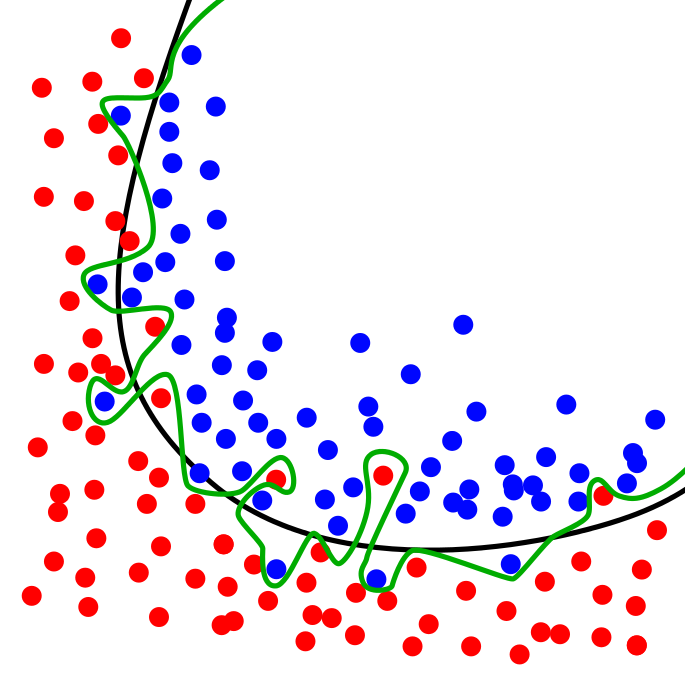
\includegraphics[width=0.5\linewidth]{overfitting.png}
\end{figure}
\end{frame}
%------------------------------------------------
\begin{frame}
\frametitle{Regularization}
\begin{itemize}
\item 
\begin{equation}
\text{min} \hspace{0.1in} J(\theta) + \lambda_C \theta^T \theta
\end{equation}
where $\lambda_C$ is the Lagrangian multiplier.
\item Lagrangian form of constrained optimization problem:
\begin{align}
\text{min} &\hspace{0.1in} J(\theta)\\
\text{s.t.} &\hspace{0.1in} \theta^T \theta \leq C
\end{align}
\end{itemize}
\end{frame}
%-------------------------------------------------
% LR and Neural networks
\subsection{To Neural networks}
\begin{frame}
\frametitle{Logistic Regression and Neural Networks}
\begin{itemize}
\item Logistic regression may be thought of as a single-layer neural network with a sigmoid activation function.
\begin{figure}
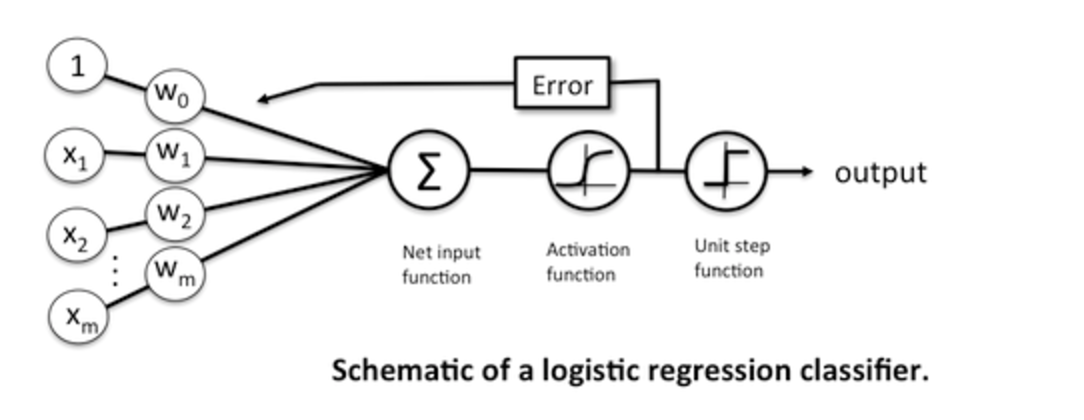
\includegraphics[width=0.8\linewidth]{LR_NN.png}
\end{figure}
\end{itemize}
\end{frame}
%------------------------------------------------
\begin{frame}
\frametitle{Logistic Regression and Neural Networks}
\begin{itemize}
\item Neural networks may be visualized as a combination of linear classifiers for complex boundaries.
\item Example: XOR function
\begin{figure}
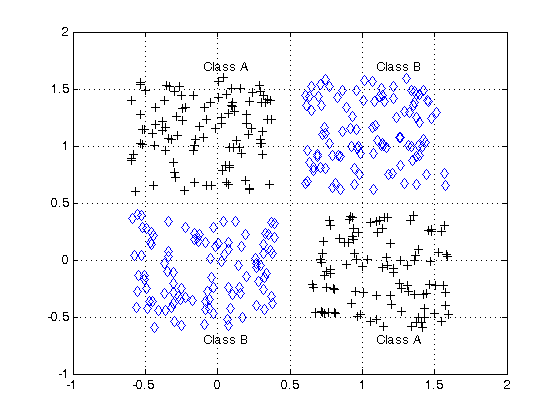
\includegraphics[width=0.6\linewidth]{xor_image.png}
\end{figure}
\end{itemize}
\end{frame}
%------------------------------------------------
\begin{frame}
\frametitle{Logistic Regression and Neural Networks}
\begin{itemize}
\item Sigmoid activation function commonly used previously in hidden layers of neural networks along with \textit{softmax} (multinomial logistic regression) at the final fully connected output layer. 
\item Nowadays, ReLU (\textbf{Re}ctified \textbf{L}inear \textbf{U}nit) activation function is most popular, but softmax is still commonly used at the final layer.
\begin{figure}
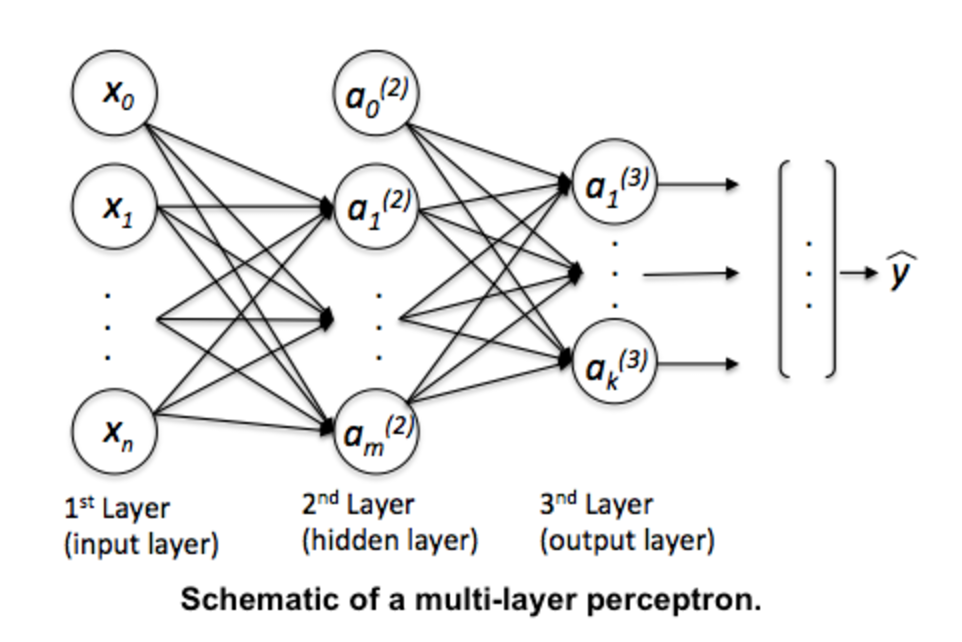
\includegraphics[width=0.5\linewidth]{MLP.png}
\end{figure}
\end{itemize}
\end{frame}
%------------------------------------------------
\begin{frame}
\frametitle{Logistic Regression and Neural Networks}
\begin{itemize}
\item Logistic regression cost function is convex, but cost function of neural networks is non-convex due to combination of multiple logistic regression layers.
\begin{figure}
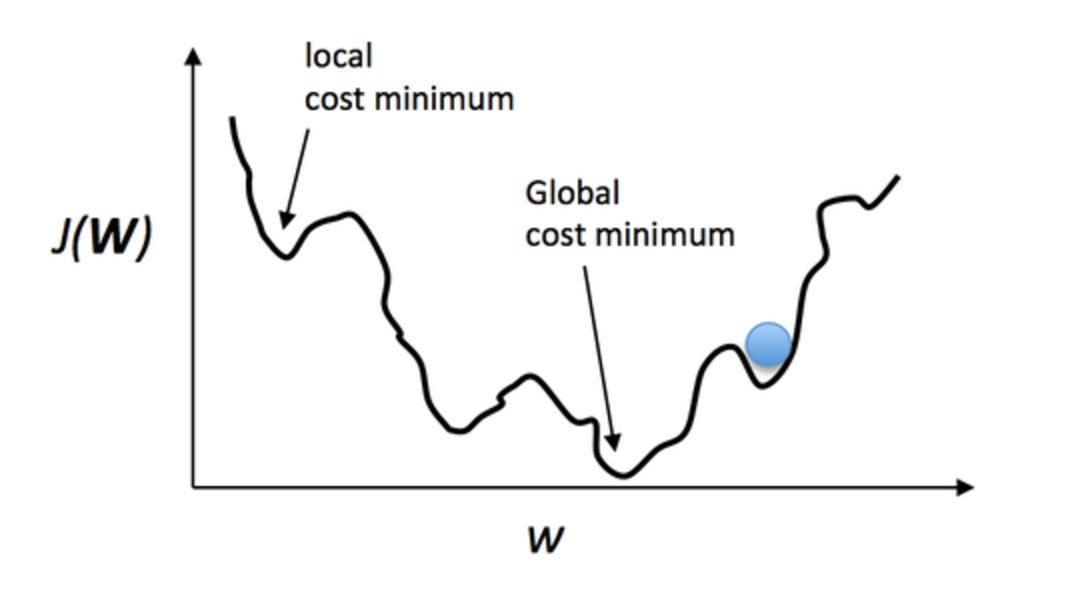
\includegraphics[width=0.7\linewidth]{NN_cost.png}
\end{figure}
\end{itemize}
\end{frame}
%%%%%%%%%%%%%%%%%%%%%%%%%%%%%%%%%%%%%%%%%%%%%%%%%%%%%%%%%%%%%%%%%%%%%%
% LaTeX Template: Beamer arrows
%
% Source: http://www.texample.net/
% Feel free to distribute this template, but please keep the
% referal to TeXample.net.
% Date: Nov 2006
% 
%%%%%%%%%%%%%%%%%%%%%%%%%%%%%%%%%%%%%%%%%%%%%%%%%%%%%%%%%%%%%%%%%%%%%%
% How to use writeLaTeX: 
%
% You edit the source code here on the left, and the preview on the
% right shows you the result within a few seconds.
%
% Bookmark this page and share the URL with your co-authors. They can
% edit at the same time!
%
% You can upload figures, bibliographies, custom classes and
% styles using the files menu.
%
% If you're new to LaTeX, the wikibook is a great place to start:
% http://en.wikibooks.org/wiki/LaTeX
%
%%%%%%%%%%%%%%%%%%%%%%%%%%%%%%%%%%%%%%%%%%%%%%%%%%%%%%%%%%%%%%%%%%%%%%

%\documentclass{beamer} %
%\usetheme{CambridgeUS}
%\usepackage[latin1]{inputenc}
%\usefonttheme{professionalfonts}


%\author{Cancan Li}
%\title{Presentation title}

%\begin{document}
\section{Numerical Optimization } 
\begin{frame}
\huge{\centerline{Section 3: Optimization Methods}}
\end{frame}

\begin{comment}
:Title: Beamer arrows
:Tags: Remember picture, Beamer, Physics & chemistry, Overlays
:Use page: 3

With PGF/TikZ version 1.09 and later, it is possible to draw paths between nodes across
different pictures. This is a useful feature for presentations with the
Beamer package. In this example I've combined the new PGF/TikZ's overlay feature
with Beamer overlays. Download the PDF version to see the result.

**Note.** This only works with PDFTeX, and you have to run PDFTeX twice.

| Author: Kjell Magne Fauske

\end{comment}


% For every picture that defines or uses external nodes, you'll have to
% apply the 'remember picture' style. To avoid some typing, we'll apply
% the style to all pictures.
\tikzstyle{every picture}+=[remember picture]

% By default all math in TikZ nodes are set in inline mode. Change this to
% displaystyle so that we don't get small fractions.
\everymath{\displaystyle}



\begin{frame}
\frametitle{What Optimization Methods to Use?}

\begin{itemize}
\item Cost function of Logistic Regression is convex
\end{itemize}

\end{frame}





\begin{frame}
\frametitle{Newton's Method for Optimization}

\tikzstyle{na} = [baseline=-.5ex]

\begin{itemize}
    \item  Newton's Method in 1-D is used as an approximation tool to find roots of differentiable functions
      \begin{itemize}
       \item Second order Taylor Expansion $\ell^T(\theta)$ of $\ell$ around $\theta_n$
       \begin{equation}
       \theta_{n+1} = \theta_n - \frac{\ell^{'}(\theta)}{\ell^{''}(\theta)}
       \end{equation}
      \end{itemize}
    \end{itemize}

    \begin{figure}[!h]
\begin{center}
%\vspace{10cm}
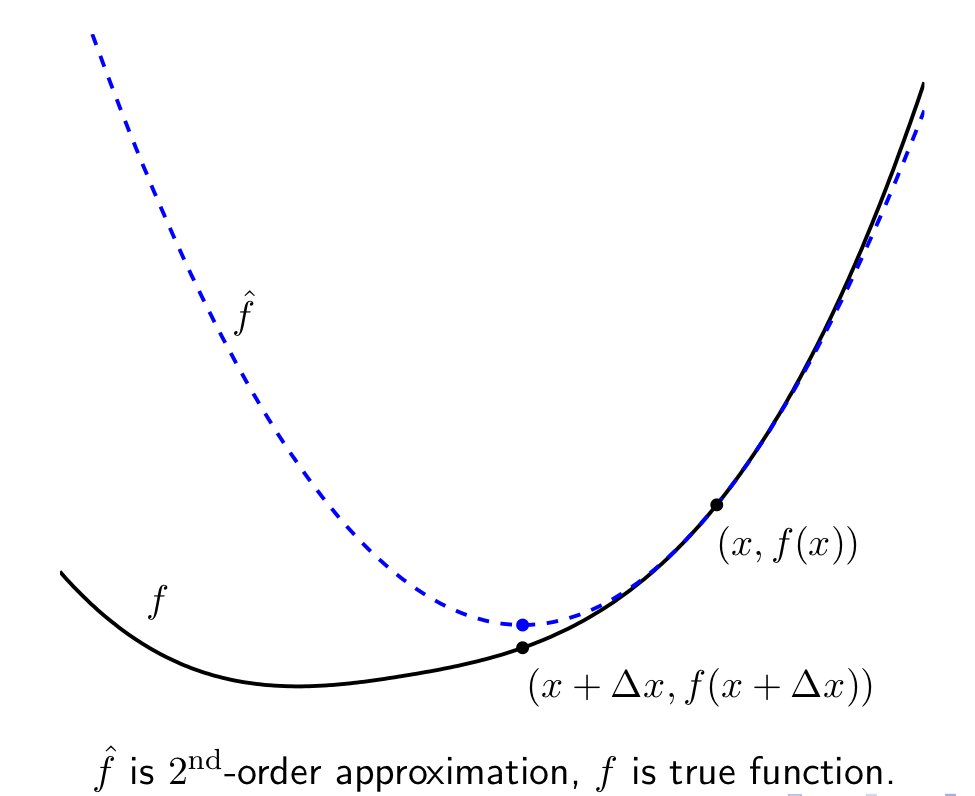
\includegraphics[width=5.5cm]{f1.png}
\end{center}
%\caption{visual representation of desired homotopy}
\label{12345678 figure name }%%%%%
\end{figure}

\end{frame}
%\frametitle{Newton's Method for Optimization}
%%%%%%%%%%%%%%%%%%%%%%%%%%%%%%%page 2 %%%%%%%%%%%%%%


 
 
\begin{frame}
\frametitle{Newton's Method in Higher Dimensions}
\begin{itemize}
       \item When $l$ is a function of multiple arguments
       \begin{center}
       $\theta_{n+1} = \theta_n - H^{-1} (\theta_n) \delta \ell(\theta_n)$
       \end{center}
       \item Calculating the inverse of $H$ is very time consuming 
        
   \end{itemize}
  \end{frame}
    




\begin{frame}
\begin{itemize}
    \item Pros 
    \begin{itemize}
    \item Converge quadratically
    \item Finds minima instead of general critical points
       \end{itemize}
        
            \item Cons 
               \begin{itemize}
               \item Newton's Method uses second partial derivatives, which may be complex to calculate
               \item Hessian matrix requires $O(n^3)$ operations to solve and $O(n^2)$ memory to store
               \item Newton's Method may diverge away from the root if the initial point is chosen poorly 
       \end{itemize}
          \end{itemize}
  \end{frame}





\begin{frame}
\frametitle{Newton's Method for Optimization}
\begin{itemize}
    \item  Because of the problems that Newton's Method has, We used Gradient Descent to minimize our cost function 
    \\
\begin{center}

  \end{center}
 
   \end{itemize}   
  \end{frame}
 



\begin{frame}
\frametitle{Gradient Descent}
\begin{itemize}

\item Having an estimate of $\delta \ell$, gradient of a function $\ell$ 
\item Decrease $\ell$ by a quantity along the direction of $\delta \ell$
  \begin{itemize}
  \item Direction
  \item Step size
  \end{itemize}
\item https://www.youtube.com/watch?v=GCvWD9zIF-s
\end{itemize}

\end{frame}



          

\begin{frame}
\frametitle{Quasi-Newton Method}

\begin{itemize}
\item Used when the problem size is big and the Hessian matrix is dense
\item Keeps "a rolling estimate" of $H(x)$ to solve this problem
\end{itemize}

  \end{frame}
  
% Newton's method as Iteratively Re-weighted Least Squares
% Frame 1
\begin{frame}
\frametitle{Newton's Method as Iteratively Re-weighted Least Squares}
\begin{itemize}
\item Recall, logistic regression model is a Bernoulli distribution with parameter $\sigmoid$:

\begin{equation}
\begin{split}
P(Y=y|X=\mathbf{x},\theta) &= \sigmoid^y (1 - \sigmoid)^{1-y}\\
&= \text{Ber}(y; \sigmoid)
\end{split}
\end{equation}

\item Again, logistic regression may be formulated as linear regression that best fits the \textit{log-odds}:
\begin{equation}
\begin{split}
\log \frac{P(Y=1|X=\mathbf{x},\theta)}{P(Y=0|X=\mathbf{x},\theta)} &= \log \frac{\sigmoid}{1 - \sigmoid}\\
&= \theta^T \mathbf{x}
\end{split}
\end{equation}

\end{itemize}
\end{frame}

% Frame 2
\begin{frame}
\frametitle{Newton's Method as Iteratively Re-weighted Least Squares}
\begin{itemize}
\item Linear regression is heavily affected by outliers - all observation variables may not have same precision of measurement (or \textit{variance}).
\item \textit{Weighted least squares} associates amount of $uncertainty$ at every point as a weight - large weights on points with \textit{high precision} or \textit{low variance} and vice-versa.
\item \textbf{Idea:} Multiply squared distance at each observation point by inverse of variance.
% Draw on board
\end{itemize}
\end{frame}

% Frame 3
\begin{frame}
\frametitle{Newton's Method as Iteratively Re-weighted Least Squares}
\begin{itemize}
\item Illustration:
\end{itemize}

\begin{figure}
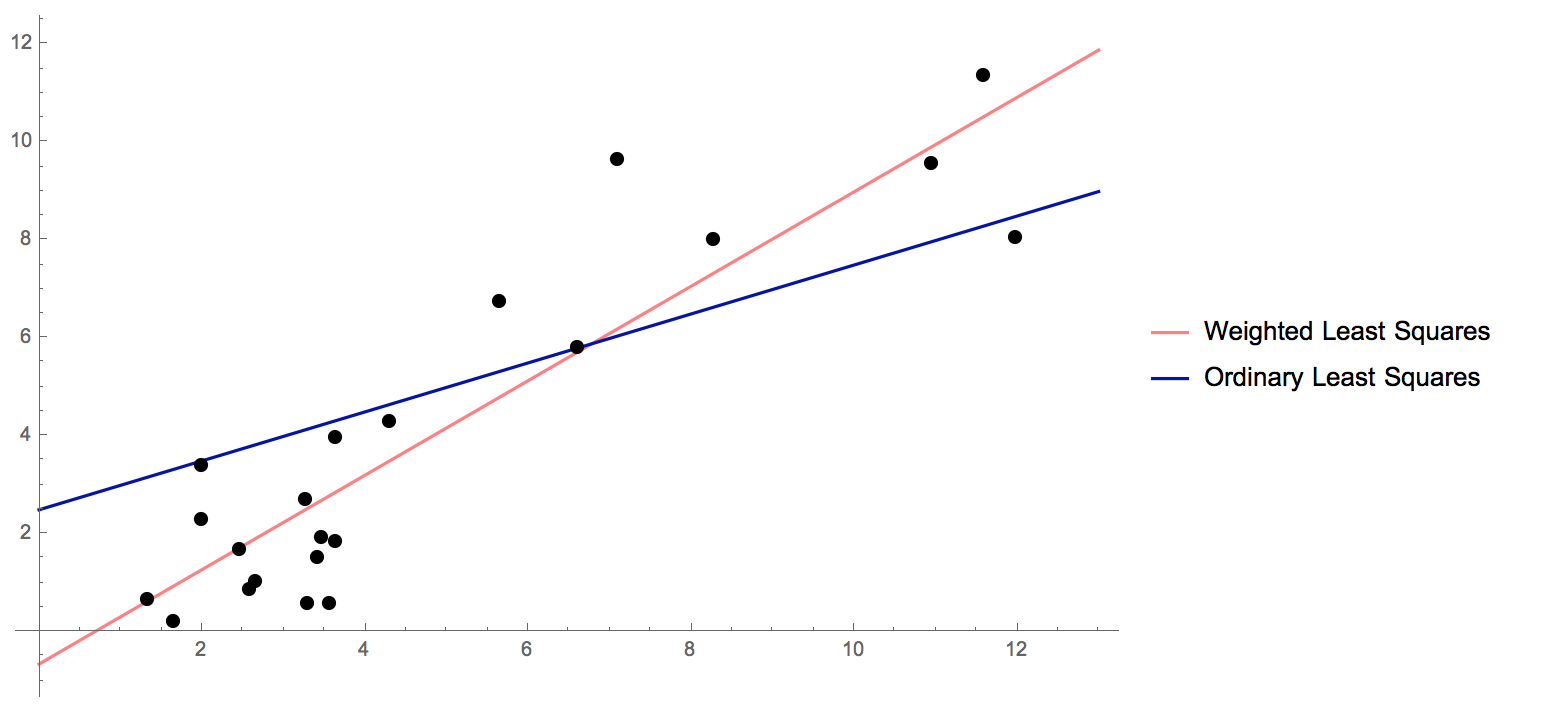
\includegraphics[scale = 0.4]{weightedLS}
\end{figure}
\end{frame}

% Frame 4
\begin{frame}
\frametitle{Newton's Method as Iteratively Re-weighted Least Squares}
\begin{itemize}
\item Loss function for weighted least squares regression (without regularization):
\begin{equation}
\mathcal{L(\theta)} = \sum_{i=1}^n \frac{1}{\text{Var}(y_i)}(y_i - \theta^T x_i)^2
\end{equation}
\item Least squares solution ($\text{Var}(y_i) = \text{const.})$:
\begin{equation}
\theta^* = (X^TX)^{-1}X^TY
\end{equation}
where $X = [x_1,...,x_n]^T, Y = [y_1,...,y_n]^T$.
\end{itemize}
\end{frame}

% Frame 5
\begin{frame}
\frametitle{Newton's Method as Iteratively Re-weighted Least Squares}
\begin{itemize}
\item \textit{Weighted} least squares solution:
\begin{equation}
\theta^* = (X^T WX)^{-1}X^T WY
\end{equation}
with $n \times n$ diagonal matrix $W_{ii} = \frac{1}{\text{Var}(y_i)}$
\item Variance of a Bernoulli distribution with parameter $p$ is $p(1-p)$. Hence, for logistic regression model,
\begin{equation}
W_{ii} = \frac{1}{\sigma (\theta^T x_i) (1 - \sigma (\theta^T x_i))}
\end{equation}
\end{itemize}
\end{frame}


% Frame 6
\begin{frame}
\frametitle{Newton's Method as Iteratively Re-weighted Least Squares}
\begin{itemize}
\item It can be shown that \textit{in expectation}, a step update by Newton's method on the logistic regression objective function is equivalent to reaching the weighted least-squares solution.
\item \textbf{Key reason}: Expected second derivative of the Bernoulli log-likelihood function is inversely proportional to the variance of the Bernoulli distribution (proof not shown).
\item However, not a single-step solution, as the weights themselves are functions of $\theta$ and the objective function is not quadratic.

%\item It can be shown that the Hessian matrix $H$ for the negative log-likelihood cost function is $H = X^T WX$ (and hence it is a convex function).
%\item Replacing $H$ and deriving the gradient from the weighted least-squares objective function, 
\end{itemize}
\end{frame}
  
  

%\end{document}
\section{Generalized Linear Models and Generalized Additive Models}
\begin{frame}
\huge{\centerline{Section 4: Generalized Linear Models }}
\huge{\centerline{and Generalized Additive Models}}
\end{frame}

\begin{frame}
\frametitle{Generalized Linear Models (GLM)}
\begin{itemize}
\item Generalized Linear Models are models in which conditional distribution of the response falls in some parametric family (exponential family), and the parameters are set by the linear predictor.
\item Link function determines the relationship between the parameters and the linear predictor.
\item Usually $g(E(\textbf{Y}))=g(\textbf{$\mu$})=\textbf{$X$}\textbf{$\theta_1$}+\textbf{$\theta_0$}$, where g is the link function.
\end{itemize}
\end{frame}

\begin{frame}
\frametitle{Generalized Linear Models (GLM) }
\begin{itemize}
\item Both least-squares regression and logistic regression are part of generalized linear models. 
\item Least-squares regression assumes gaussian distribution with mean predicted by the linear predictor. (identity link)
\item Logistic regression assumes binomial distribution, with $n$ equal to the number of data points with given $x$, and $p$ given by the logistic function. $(p=\frac{1}{1+e^{-(\theta_0+x \cdot \theta_1)}})$
\end{itemize}
\end{frame}
%\begin{frame}
%\frametitle{Linear Predictors}
%\begin{itemize}
%\item Maybe we don't need the slide
%\end{itemize}
%\end{frame}

% \begin{frame}
% \frametitle{Link Function}
% \begin{itemize}
% \item Link function determines the relationship between the parameters and the linear predictor.
% \item For GLM, link function may be any monotonic differentiable function. 
% \end{itemize}
% \end{frame}

\begin{frame}
\frametitle{GLM vs LM}
Data is generated with the the equation $y\sim \mathcal{N}(\mu, 0.5)$, $\mu=\frac{1}{0.4x}$.
\begin{figure}
\centering
\begin{subfigure}{.5\textwidth}
  \centering
  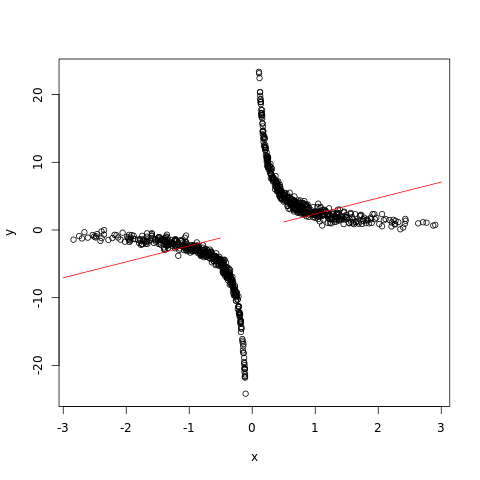
\includegraphics[height=.5\textheight]{glm/Unknown-2}
  \caption{Line fitted with least regression}
  \label{fig:sub1}
\end{subfigure}%
\begin{subfigure}{.5\textwidth}
  \centering
  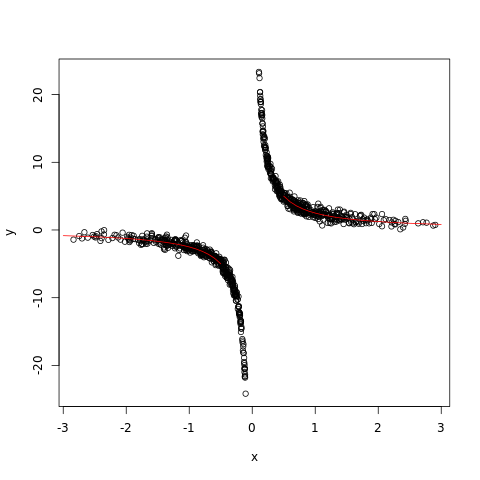
\includegraphics[height=.5\textheight]{glm/Unknown3}
  \caption{Line fitted with GLM}
  \label{fig:sub2}
\end{subfigure}
\label{fig:test}
\end{figure}
\end{frame}

\begin{frame}
\frametitle{Generalized Additive Models (GAM) }
\begin{itemize}
\item Unlike Generalized Linear Models, instead of making the transformed mean a linear function of the inputs, we can make it an additive function of the inputs
\item $g(E(\textbf{Y}))=g(\textbf{$\mu$})=\alpha + f_1(x_1) + f_2(x_2) + ... + f_n(x_n)$
\end{itemize}
\end{frame}

\begin{frame}
\frametitle{Model Checking}
\begin{itemize}
\item When our GLM is wrong, then no matter how much data we use, the prediction of our model is systematically wrong. However, since GAM can be nonparametric, with enough data, GAM will fit better than GLM. We can therefore use this property to design a procedure that detect if our GLM is wrong.
\end{itemize}
\end{frame}

\begin{frame}
\frametitle{Model Checking}
$MSE$: Mean Squared Error \\
$MSE_{p}$: Parametric mean squared error \\
$MSE_{np}$: Nonparametric \\
\begin{enumerate}
\item Fit a GAM and a GLM to the same data. Compute $MSE_p$ and $MSE_{np}$. Compute $t = MSE_p - MSE_{np}$.
\item Simulate from fitted GLM, refit both models to the simulated data. Repeat many times. compute $\hat{MSE_p}$ and $\hat{MSE_{np}}$. Compute $\hat{t} = \hat{MSE_p} - \hat{MSE_{np}}$.
\item p-value: $\frac{1 + \#\{\hat{t} > t\}}{1+\#\hat{t}}$
\end{enumerate}
\end{frame}

\begin{frame}
\frametitle{Model Checking: Example}
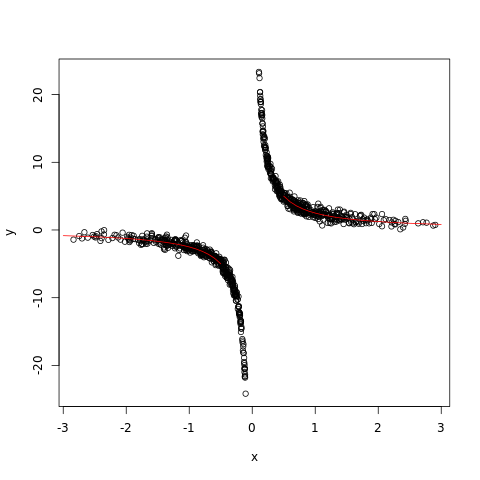
\includegraphics[height=.5\textheight]{glm/Unknown3}
\begin{itemize}
\item By performing model checking on our glm model with inverse link function, we get p-value of 0.72. This is reassuring, since the data is indeed generated from the inverse of a linear function.
\end{itemize}
\end{frame}

% \begin{frame}
% \frametitle{Trivia}
% \begin{itemize}
% \item Note that when the training data is perfectly linearly separable, maximum likelihood works badly for GLM.
% \end{itemize}
% \end{frame}
%------------------------------------------------
%-----session 5: Applications, Chih Yun Pai------
%------------------------------------------------

\section{Applications}
\begin{frame}
\huge\frametitle{Section 5: Applications}
\centering
Section 5: Applications
\par
\end{frame}
%------------------------------------------------
%Quick Review
%------------------------------------------------
\begin{frame}
\frametitle{Quick Review}

What we get so far... \newline\newline

Logistic Regression hypothesis: $h_\theta(x)=\frac{1}{1+e^{-\theta^Tx}}$\newline\newline

Optimization: Gradient Descent / Newton Method\newline\newline

Regularization\newline\newline

\end{frame}

%------------------------------------------------
%Logistic Regression as binary classifier-1
%------------------------------------------------
\subsection{LR for Linearly Separable Dataset}
\begin{frame}
\frametitle{Logistic Regression as Binary Classifier}
Problem: Predict whether a student gets admitted into a university, given two historical exams data.\newline\newline
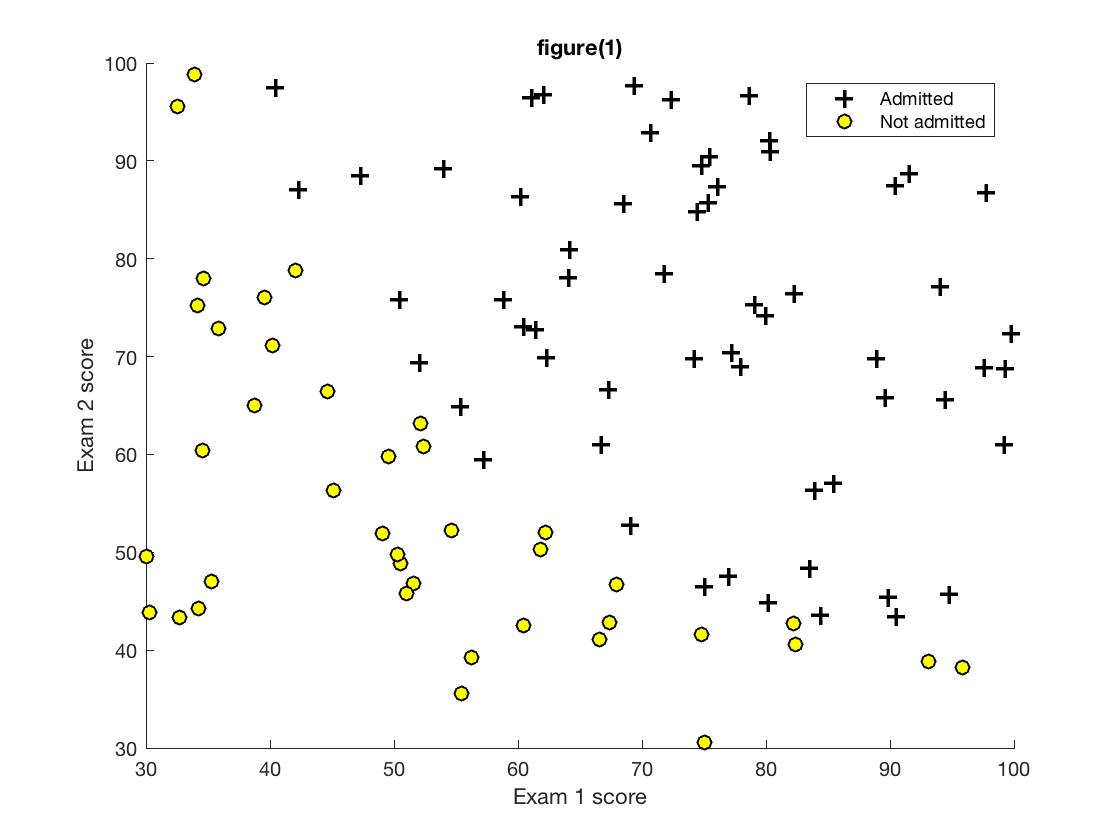
\includegraphics[width=4cm,height=5cm,keepaspectratio]{pictures/1_plotData1}\newline
Labels: y=1: Admitted / y=0: Not admitted\newline\newline
Logistic model: $h_\theta(x)=\frac{1}{1+e^{-\theta^Tx}}$\newline\newline
\end{frame}

%------------------------------------------------
%Logistic Regression as binary classifier-2
%------------------------------------------------
\subsection{LR for Nonlinearly Separable Dataset}
\begin{frame}
\frametitle{Logistic Regression as Binary Classifier}
Cost function without regularization: \newline\newline
$J(\theta)=\frac{1}{n}\sum\limits_{i=1}^n[-y^{(i)}*log(h_\theta(x^{(i)}))-(1-y^{(i)})*log(1-h_\theta(x^{(i)})]$\newline\newline
Optimized by Gradient Descent\newline\newline
Training Accuracy: 89\%
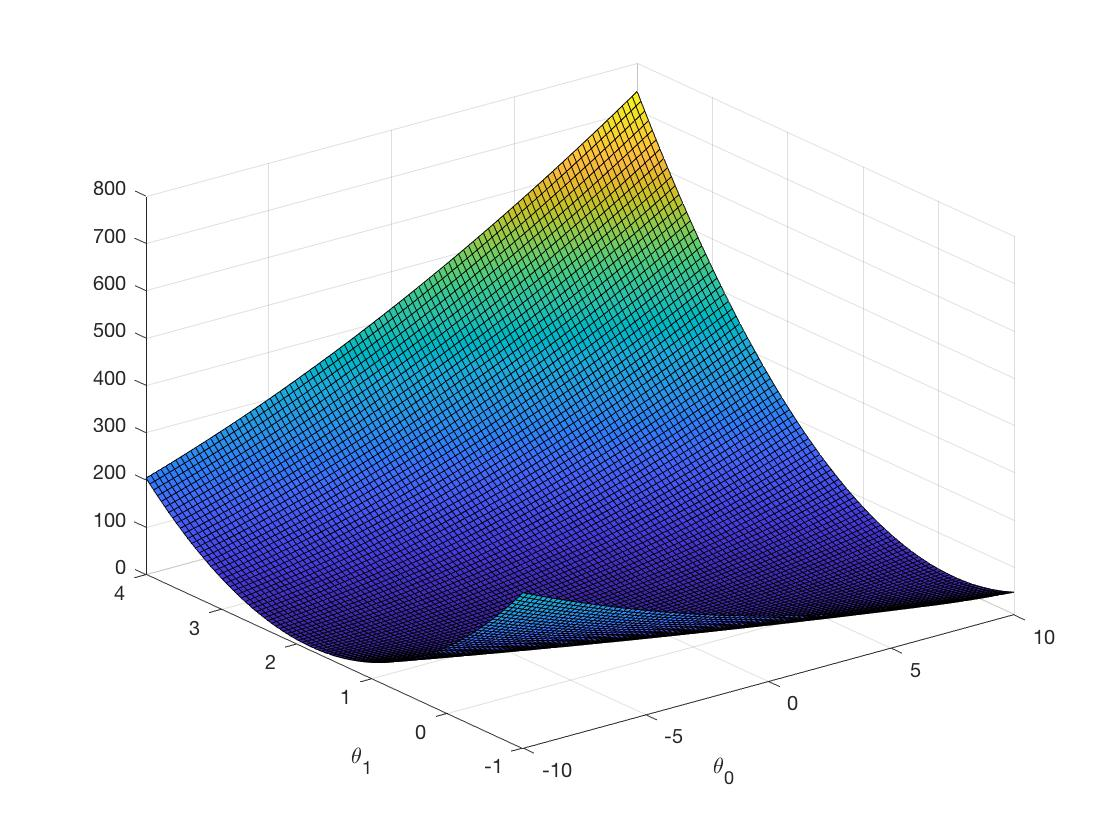
\includegraphics[width=5cm,height=5cm,keepaspectratio]{pictures/0_optimization_result_in_3-d_graph}
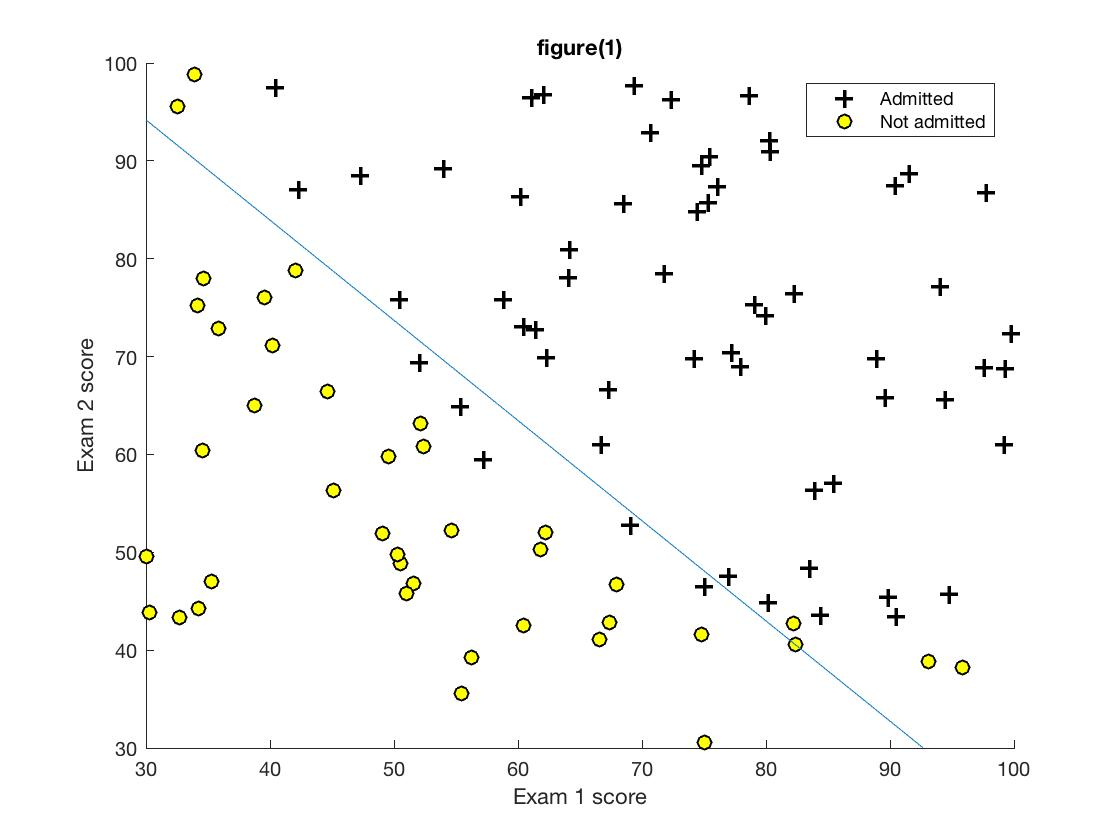
\includegraphics[width=5cm,height=5cm,keepaspectratio]{pictures/2_plotData1_decision_boundary}
\end{frame}

%------------------------------------------------
%Logistic Regression as binary classifier with Regularization-1
%------------------------------------------------
\begin{frame}
\frametitle{Logistic Regression as Binary Classifier with Regularization}
Problem: Predict whether a product of Microchip Manufacturing is malfunction, given 2 kind of tests score. Labels: y=1 pass / y=0 fail.\newline\newline
Logistic model: $h_\theta(x)=\frac{1}{1+e^{-\theta^Tx}}$\newline\newline
Cost function with regularization: \newline\newline
$J(\theta)=\frac{1}{n}\sum\limits_{i=1}^n[-y^{(i)}*log(h_\theta(x^{(i)}))-(1-y^{(i)})*log(1-h_\theta(x^{(i)})]+\frac{\lambda}{2n}\sum\limits_{j=1}^d\theta_j^2$\newline\newline
Feature Transformation: $Z(x)=[1,x_1,x_2,x_1^2,x_2^2,x_1x_2,...,x_1x_2^5,x_2^6]^T$\newline\newline
Optimized by Gradient Descent\newline\newline

\end{frame}

%------------------------------------------------
%Logistic Regression as binary classifier with Regularization-2
%------------------------------------------------
\begin{frame}
\frametitle{Logistic Regression as Binary Classifier with Regularization}

Training Accuracy: \newline\newline

\begin{figure}[h!]

\begin{subfigure}{.3\textwidth}
  \centering
  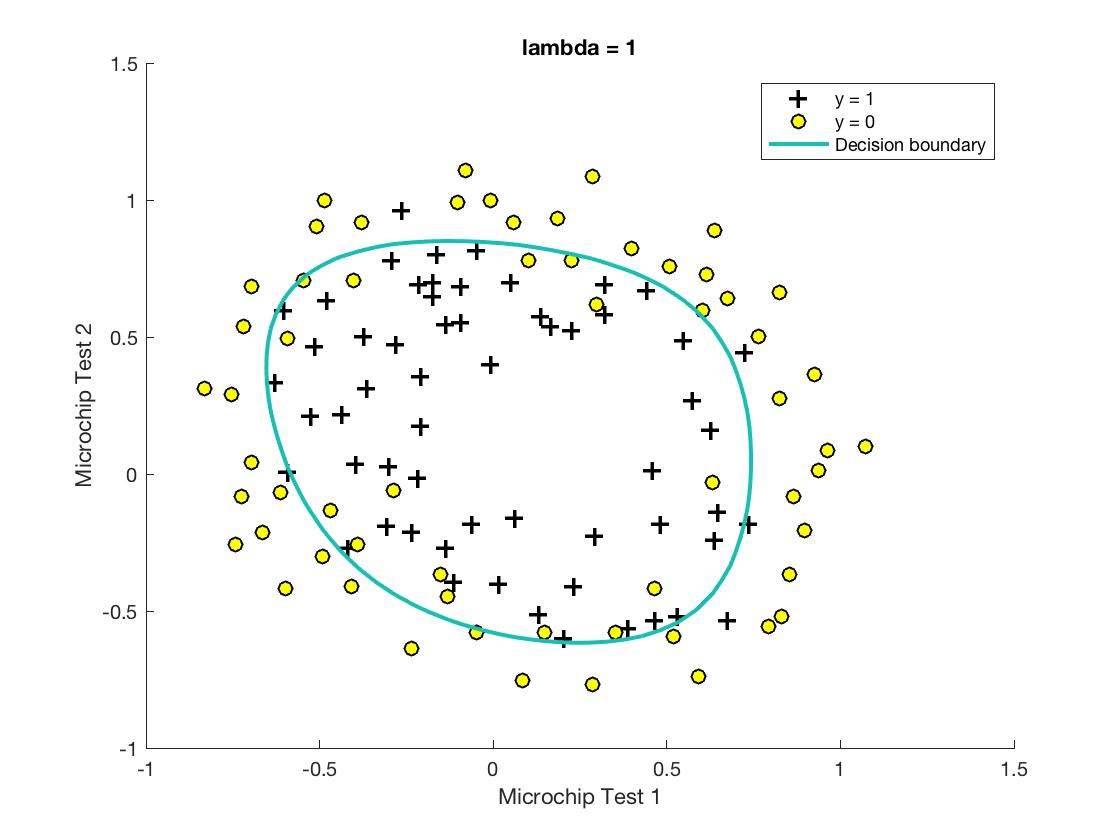
\includegraphics[scale = 0.1]{pictures/4_plotData2_lambda_1}
  \caption{$\lambda=1$:\\ accuracy = 83\% \\ Good fitting}
  \label{fig:sub1}
\end{subfigure}
\begin{subfigure}{.3\textwidth}
  \centering
  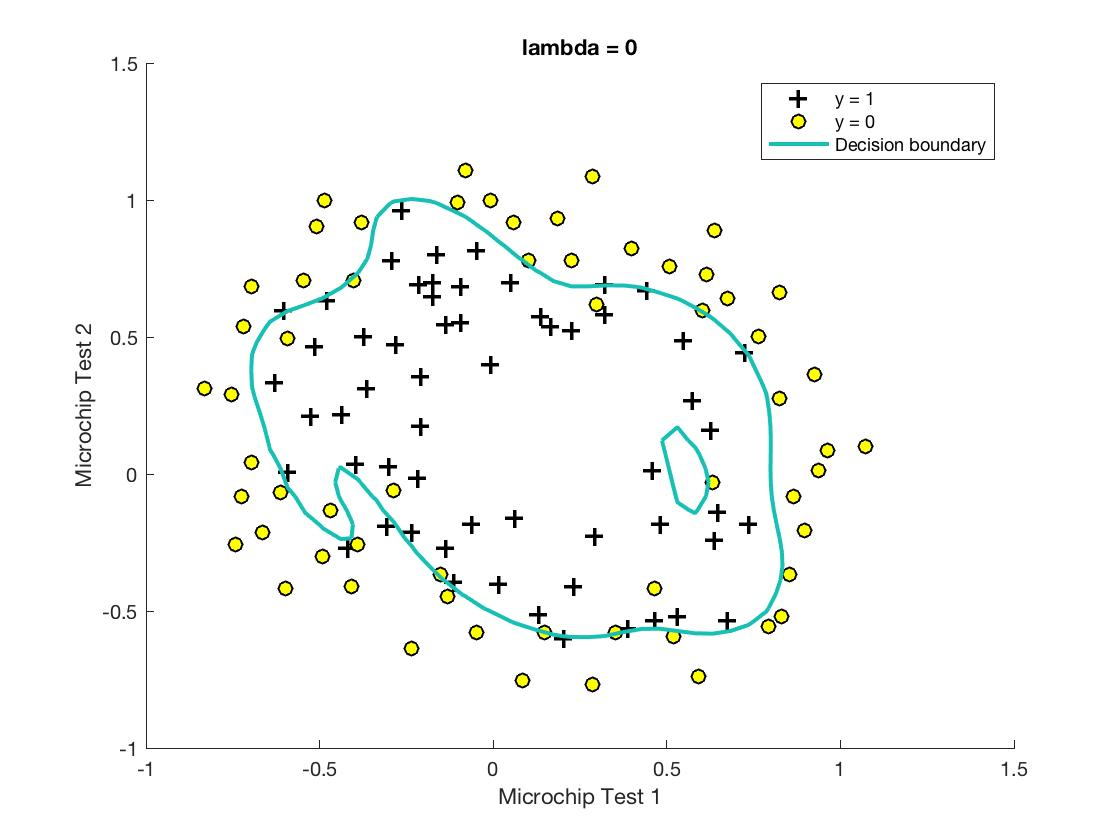
\includegraphics[scale = 0.1]{pictures/5_plotData2_lambda_0_overfitting}
  \caption{$\lambda=0$:\\ accuracy = 87\% \\ Over-fitting}
  \label{fig:sub2}
\end{subfigure}
\begin{subfigure}{.3\textwidth}
  \centering
  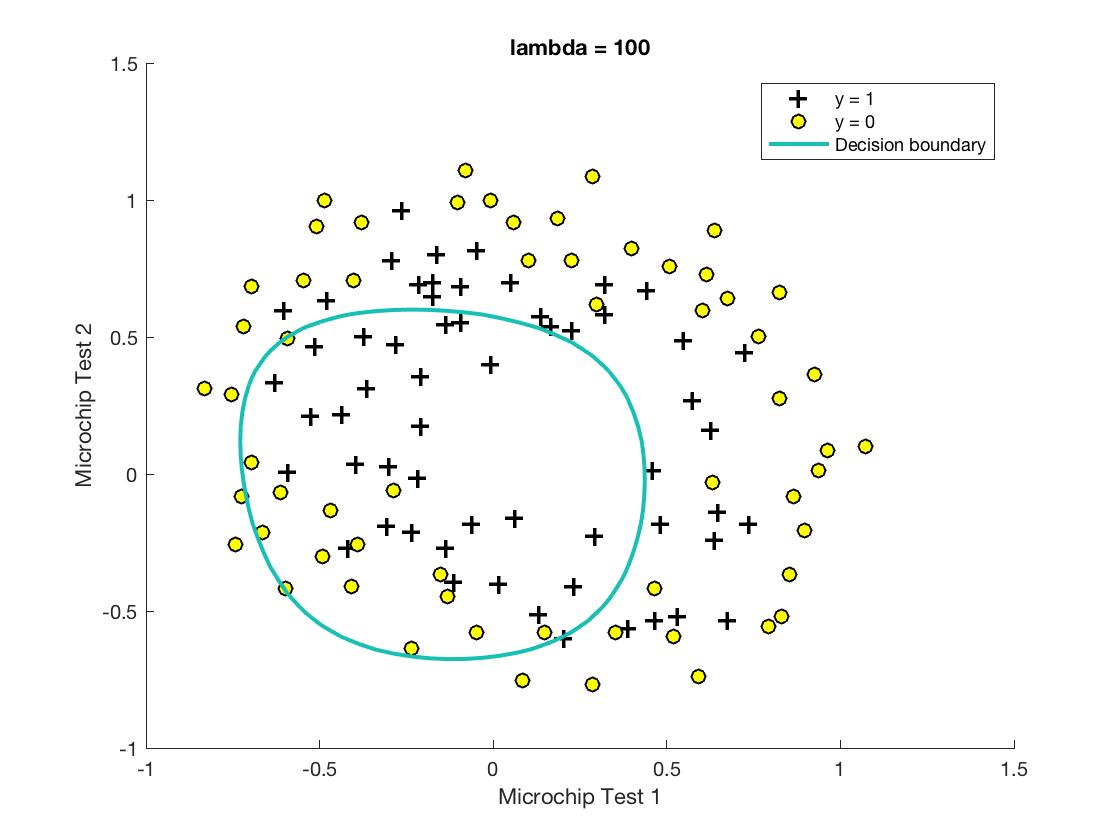
\includegraphics[scale = 0.1]{pictures/6_plotData2_lambda_100_underfitting}
  \caption{$\lambda=100$:\\ accuracy = 61\% \\ Under-fitting}
  \label{fig:sub2}
\end{subfigure}
\end{figure}

\end{frame}

%------------------------------------------------
%Handwritten Digit Recognition
%------------------------------------------------
\subsection{Applications: Handwritten Digit Recognition}
\begin{frame}
\frametitle{Handwritten Digit Recognition}
Problem: Recognize handwritten digits (from 0-9)\newline\newline
Dataset: 5000 20 pixel by 20 pixel greyscale images, 5000 labels \newline\newline
X: 5,000 $\times$400 matrix\newline\newline
Y: 5,000 $\times$1 vector $\in {0,1,...,9}$
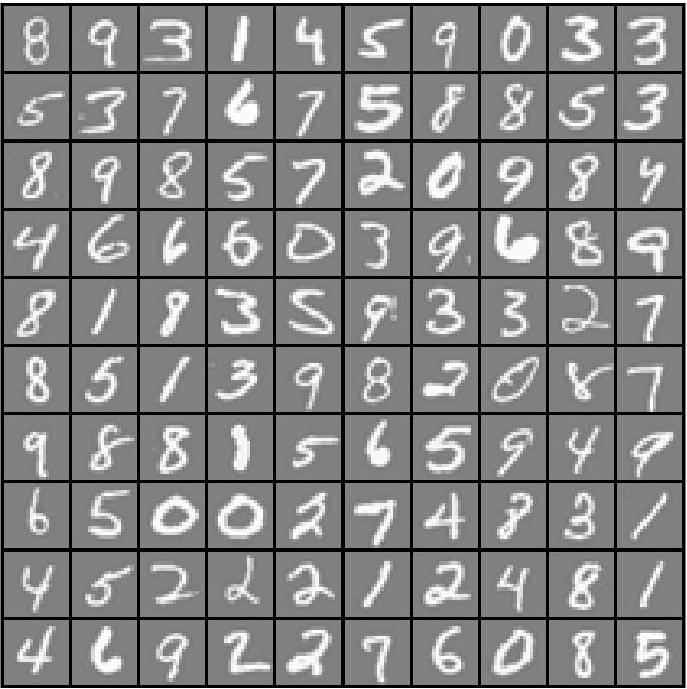
\includegraphics[width=4cm,keepaspectratio]{pictures/7_digits}
\end{frame}

%------------------------------------------------
%Handwritten Digit Recognition - Model
%------------------------------------------------

\begin{frame}
\frametitle{Handwritten Digit Recognition - Model}
Model:\newline
- Logistic Regression hypothesis: $h_\theta(x)=\frac{1}{1+e^{-
\theta^Tx}}$\newline
- One vs All multi-class classification: $h_\theta^{(c)}=P(y=c|x;\theta), c=1,...,10$\newline
- Prediction: $\underset{c}max$ $h_\theta^{(c)}(x)$\newline
- Neural Network  (one hidden layer, 25 units), Optimization: Back-propagation with Gradient Descent\newline
\begin{centering}
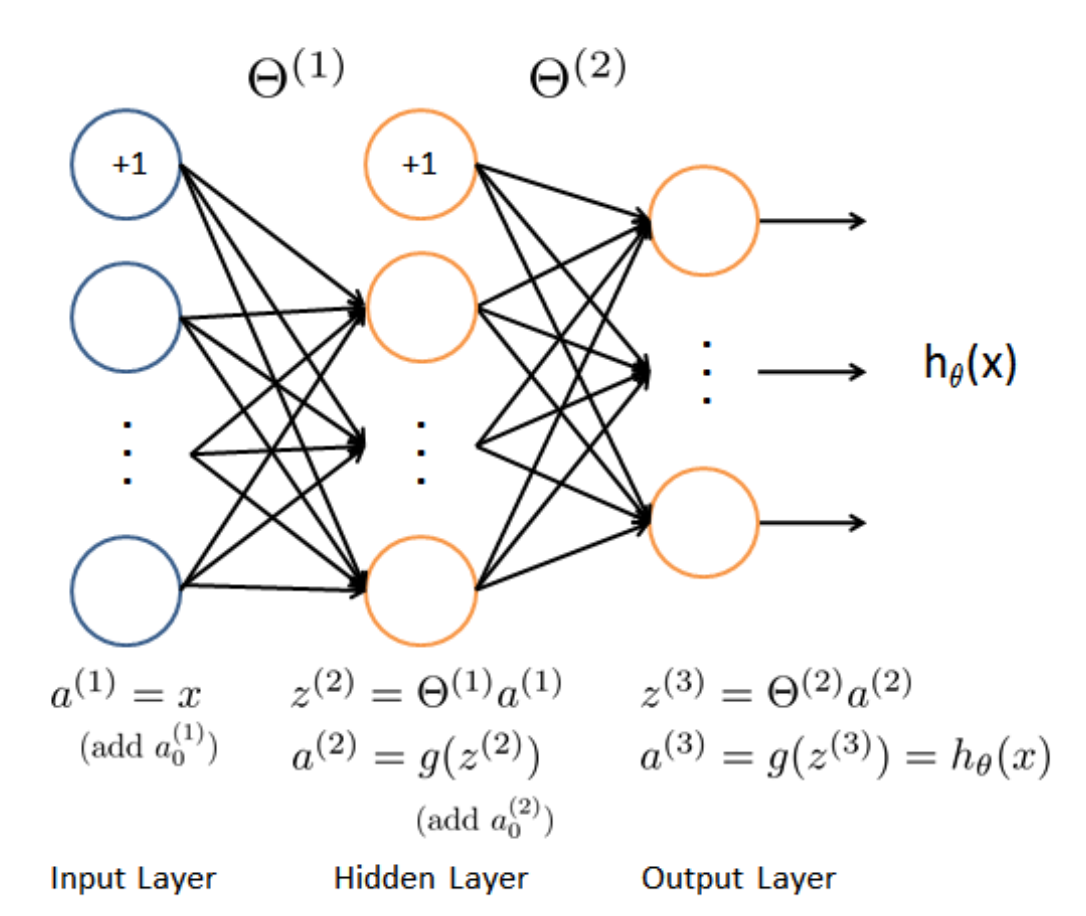
\includegraphics[width=5cm,keepaspectratio]{pictures/8_Neural_network_model}
\end{centering}
\end{frame}

%------------------------------------------------
%Handwritten Digit Recognition - Result
%------------------------------------------------
\begin{frame}
\frametitle{Handwritten Digit Recognition - Result}
\begin{itemize}
\item Hidden layer units visualization \newline\newline
\begin{figure}
\begin{centering}
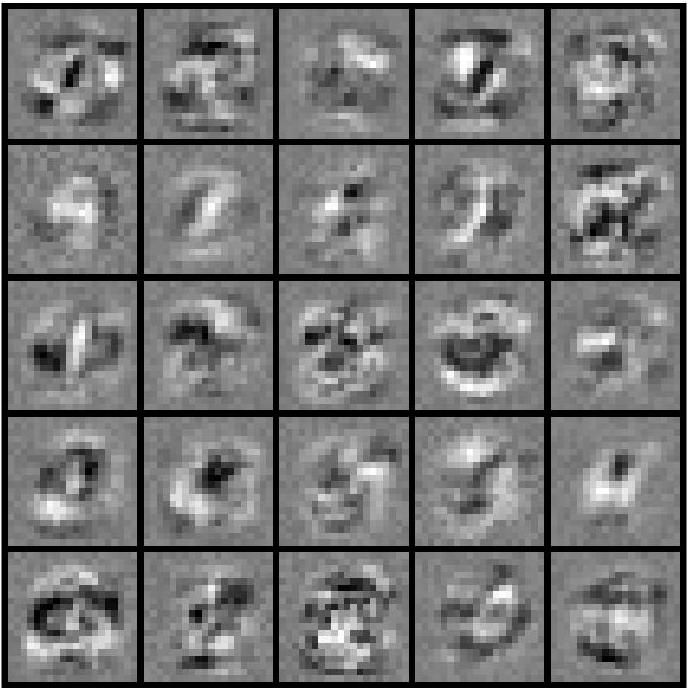
\includegraphics[width=4cm,keepaspectratio]{pictures/9_Visualizeing_hidden_layer}
\end{centering}
\end{figure}
\item Training Accuracy:\newline
97.52\% without regularization, $\lambda=0$\newline
95.36\% with regularization, $\lambda=1$ \newline
\end{itemize}
\end{frame}
%------------------------------------------------



%------------------------------------------------
%References
%------------------------------------------------
\begin{frame}
\frametitle{References}
\begin{itemize}
\item \textit{Advanced Data Analysis from an Elementary Point of View} by C. Shalizi.
\item \textit{Learning from Data} by Mostafa, Magdon-Ismail, Lin.
\item \textit{Elements of Statistical Learning} by Hastie, Tibshirani.
\item \textit{Pattern Recognition and Machine Learning} by Christopher M. Bishop.
\item \textit{A comparison of numerical optimizers for logistic regression} by Thomas P. Minka, October 22, 2003
\item CS 229 Machine Learning (Stanford) course lectures by Prof. Andrew Ng.
\item CSE 517A Machine Learning (WUSTL) course lectures by Prof. Marion Neumann.
\item Blog post by Sebastian Raschka : \url{https://sebastianraschka.com/faq/docs/logisticregr-neuralnet.html}
\end{itemize}
\end{frame}
%------------------------------------------------
%The End
%------------------------------------------------
%\section{The End}
\begin{frame}
\Huge{\centerline{Thank You!}}
\end{frame}
%------------------------------------------------
%Q&A
%------------------------------------------------
%\section{Q\&A}
\begin{frame}
\Huge{\centerline{Q\&A}}
\end{frame}


%------------------------------------------------

\end{document} 